\documentclass{article}

% Useful packages
\usepackage{amsmath}
\usepackage{graphicx}
\usepackage[colorlinks=true, allcolors=blue]{hyperref}
\usepackage{tikz}
\usepackage{tikz-3dplot}

\title{Deriving the volume formula for a cone/pyramid}
\author{Dave Neary}

\begin{document}
\maketitle

\begin{abstract}
High School Geometry students all learn the volume formula $V=\frac{1}{3}Ah$ for cones
and cylinders, where $A$ is the area of the base, and $h$ is the height of the solid. But
where does this $\frac{1}{3}$ come from?
I am going to attempt an explanation which is intuitive to a High School geometry class,
without assuming knowledge of Calculus concepts like limits and integrals.
\end{abstract}

\section*{Cavalieri's principle}

Cavalieri's principle in 3D geometry says that if you have two forms which are the same height,
and every cross-section parallel to their base has the same area, then their volumes will be
the same. Imagine, for example, that you have a pack of cards stacked in a cuboid, and then
you shift the cards slightly relative to the card underneath to make some kind of funky
twisted shape. Since the surface area of each card is identical, no matter where you cut
across the deck, and the height hasn't changed, the volume enclosed by the cards will also
be exactly the same.

\begin{figure}[h]
\centering
	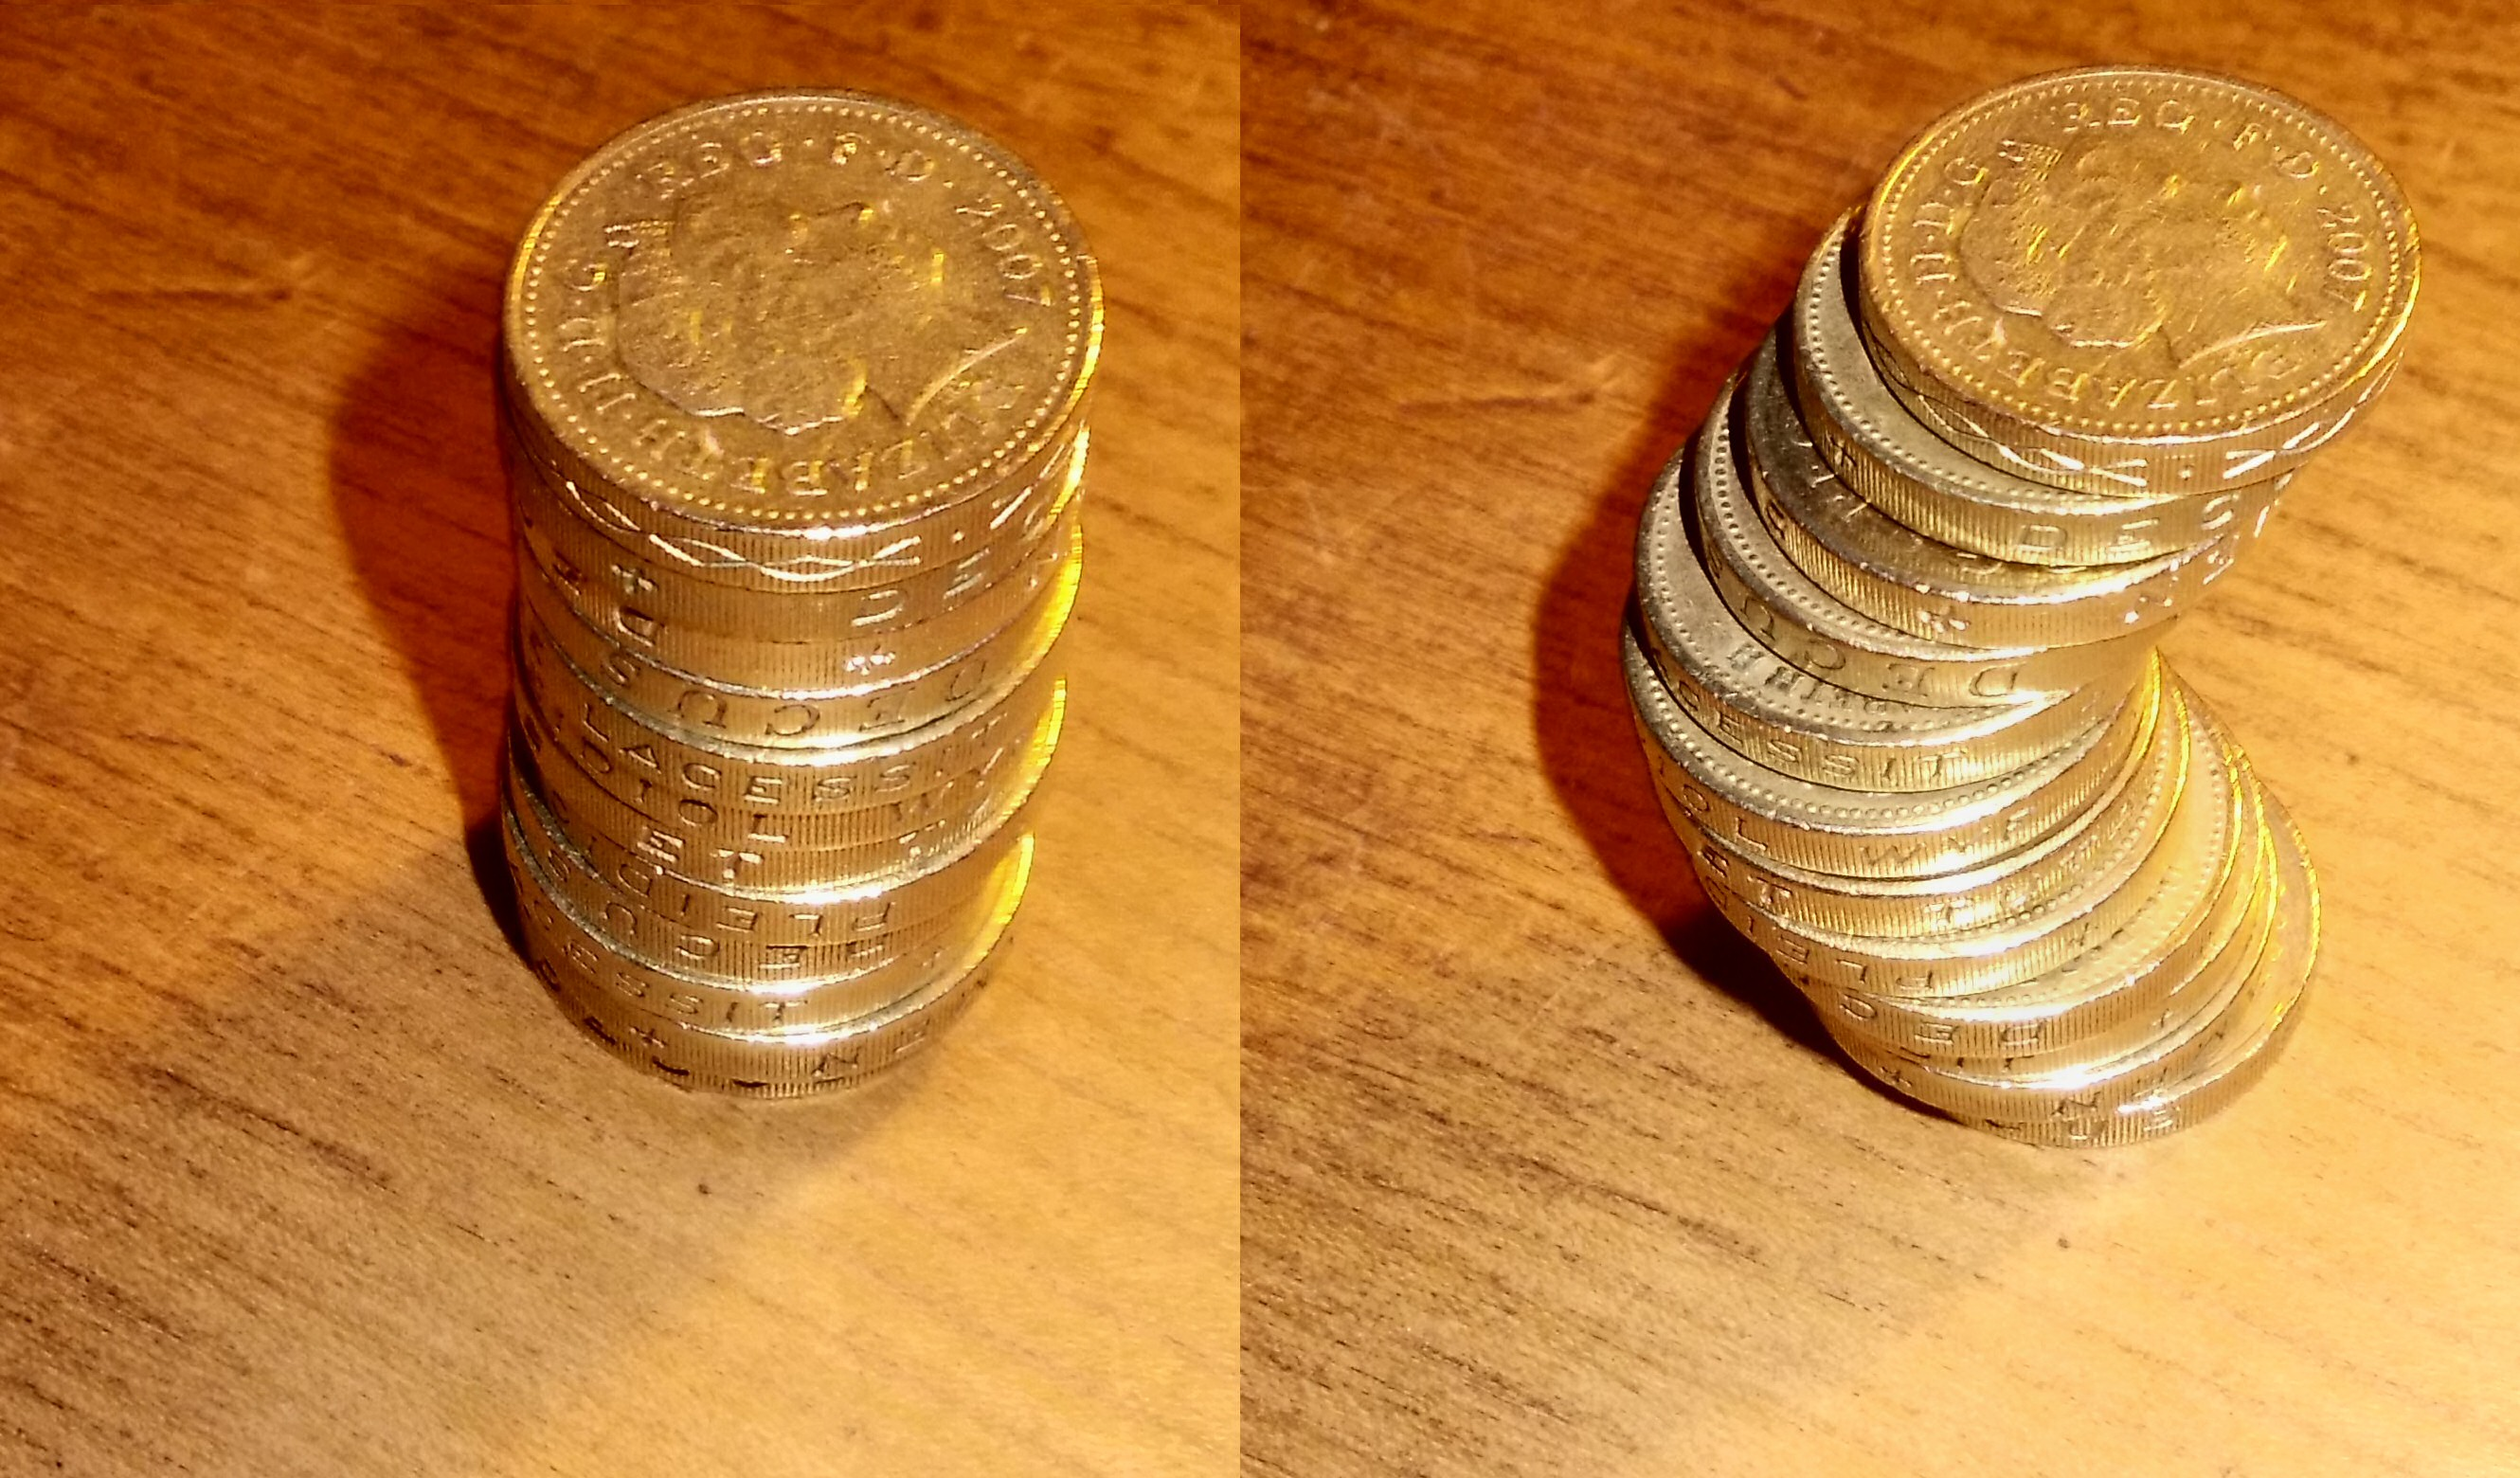
\includegraphics[width=0.5\textwidth]{Cavalieris_principle_illustration}
	\caption{Illustration of Cavalieri's principle with coins\protect\footnotemark}
\end{figure}

\footnotetext{By Chiswick Chap - Own work, CC BY-SA 3.0,
	\url{https://commons.wikimedia.org/w/index.php?curid=29718934}}

\section*{Approximation with cuboids}

To simplify our analysis, we will look at a rectangular pyramid, approximated by cuboids in two
different ways, one an under-estimate of the volume, and the other an over-estimate.
Thanks to Cavalieri's principle, we can generalize this solution to any shape, including cones.

\begin{center}
\tdplotsetmaincoords{70}{-20}
\begin{tikzpicture}[tdplot_main_coords,line cap=butt,line join=bevel]
\pgfmathsetmacro{\B}{4}
\pgfmathsetmacro{\H}{5}
 \draw[thick] (-\B/2,-\B/2,0) -- (\B/2,-\B/2,0) -- (\B/2,\B/2,0) -- (-\B/2,\B/2,0) -- cycle;
 \draw[thick] (\B/2,\B/2,0) -- (0,0,\H);
 \draw[dashed] (0,0,0) -- (0,0,\H) coordinate[midway](aux1);
 \draw (0,0,0.3) -- (0.3,0,0.3) -- (0.3,0,0);
 \coordinate (aux3) at (1,0,0);
 \draw[thick,fill=lightgray,fill opacity=0.3] (-\B/2,-\B/2,0) -- (0,0,\H) -- (\B/2,-\B/2,0) -- cycle;
 \draw[thick,fill=gray,fill opacity=0.3] (-\B/2,-\B/2,0) -- (0,0,\H) -- (-\B/2,\B/2,0) -- cycle;
 \begin{scope}[tdplot_screen_coords]
  \draw (aux1) -- ++ (2,0.1) node[right,font=\itshape] {Height};
  \draw (aux3) -- ++ (1,-1) node[below right,font=\itshape] {Base};
 \end{scope}
\end{tikzpicture}
\end{center}

Let's take a cross-section of the cone through an apex, and look at how we might
approximate its volume:

\begin{center}
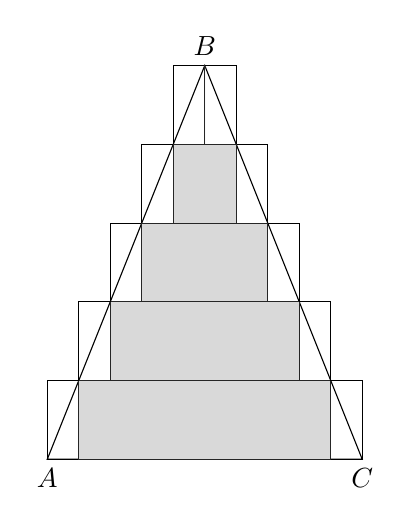
\begin{tikzpicture}
\pgfmathsetmacro{\B}{4}
\pgfmathsetmacro{\H}{5}
\pgfmathsetmacro{\DH}{1}
\pgfmathsetmacro{\DB}{\DH*\B/\H}
\pgfmathsetmacro{\STEPS}{\H/\DH}

\draw (-\B/2,0) node[anchor=north]{$A$}
  -- (\B/2,0) node[anchor=north]{$C$}
  -- (0,\H) node[anchor=south]{$B$}
  -- cycle;
\foreach \i in {1,...,\STEPS} {
  \draw (-\B/2+0.5*\i*\DB - 0.5*\DB,\i*\DH - \DH) -- (-\B/2+0.5*\i*\DB - 0.5*\DB,\i*\DH) -- (\B/2-0.5*\i*\DB + 0.5*\DB,\i*\DH) -- (\B/2-0.5*\i*\DB + 0.5*\DB,\i*\DH - \DH);
  \filldraw[fill=gray!30!white,draw=gray!30!black] (-\B/2+0.5*\i*\DB,\i*\DH - \DH) -- (-\B/2+0.5*\i*\DB,\i*\DH) -- (\B/2-0.5*\i*\DB,\i*\DH) -- (\B/2-0.5*\i*\DB,\i*\DH-\DH) -- cycle;
}
\end{tikzpicture}
\end{center}

In this figure, we see two ways that we can approximate the volume of the pyramid using
cuboids, one of which is an underestimate, and the other an overestimate. By cutting thinner slices,
we can get a good approximation of the volume of the pyramid.

If the side length of the base is $s$ (giving a base area of $s^2$), and the height is $h$, then for $n$ slices, we can find the side length of the $i$th cuboid using similar triangles. 

\begin{center}
\begin{tikzpicture}
\pgfmathsetmacro{\B}{4}
\pgfmathsetmacro{\H}{5}
\pgfmathsetmacro{\DH}{1}
\pgfmathsetmacro{\DB}{\DH*\B/\H}
\pgfmathsetmacro{\STEPS}{\H/\DH}

\draw (-\B/2,0) node[anchor=north]{$A$}
  -- (\B/2,0) node[anchor=north]{$C$}
  -- (0,\H) node[anchor=south]{$B$}
  -- cycle;

\foreach \i in {1,...,\STEPS} {
\draw (-\B/2+0.5*\i*\DB,\i*\DH) -- (\B/2-0.5*\i*\DB,\i*\DH);
}

\draw [<->] (-\B/2-0.2,0) -- node[left=1pt] {$h$} (-\B/2-0.2,\H);
\draw [<->] (0,2*\DH) -- node[left=1pt] {$\frac{h}{n}$} (0,3*\DH);
\end{tikzpicture}
\end{center}

Since all of the triangles with their apex at $B$ are similar, the base of the $i$th slice (counting from the apex) can be calculated from the similarity:

\begin{align*}
\frac{h}{s} &= \frac{\frac{ih}{n}}{s_n} \\
s_n &=\frac{i}{n}s 
\end{align*}

We can then calculate the under and overestimates of the volume by summing the volumes of the
cuboids. Since $s_i = \frac{i}{n}s$, we have $A_i = \frac{i^2}{n^2}s^2 = \frac{i^2}{n^2}A$,
the area of the base. By the way, this final statement is true not just for square pyramids, but
for any pyramid or cone - the area of a slice will always vary as the square of the scaling
factor of length in a cone.

Then:
\begin{align*}
\sum_{i=1}^{n} \frac{h}{n}A_n &> V > \sum_{i=0}^{n-1} \frac{h}{n}A_n \\
\sum_{i=1}^{n} \frac{i^2h}{n^3}A &> V > \sum_{i=0}^{n-1} \frac{i^2h}{n^3}A \\
\frac{Ah}{n^3} \sum_{i=1}^{n} i^2 &> V > \frac{Ah}{n^3} \sum_{i=0}^{n-1} i^2 \\
\frac{Ah}{n^3} \frac{(n)(n+1)(2n+1)}{6} &> V > \frac{Ah}{n^3} \frac{(n-1)(n)(2n-1)}{6} \\
\frac{Ah}{3} (1+\frac{1}{n})(1+\frac{1}{2n}) &> V > \frac{Ah}{3} (1-\frac{1}{n})(1-\frac{1}{2n})
\end{align*}

For this, we use the formula:
\[ \sum_{i=1}^{n} i^2 = \frac{(n)(n+1)(2n+1)}{6} \]
which we can prove by induction, and we simplify the expressions afterwards by dividing each term
in the numerator by one of the $n$s in the denominator, and finally writing $2-\frac{1}{n} = 2(1-\frac{1}{2n})$ to get our final expression.

It is easy to see that as we take more and more slices, the lower bound and the upper bound both
get closer and closer to $\frac{Ah}{3}$, one from below, and the other from above. Since we can
increase the number of slices we take arbitrarily, this is thus the exact volume of the pyramid,
and by Cavalieri's principle, this is also the volume of any pyramidal shape, including cones.

\end{document}


